
    \begin{figure}[]
        \centering
		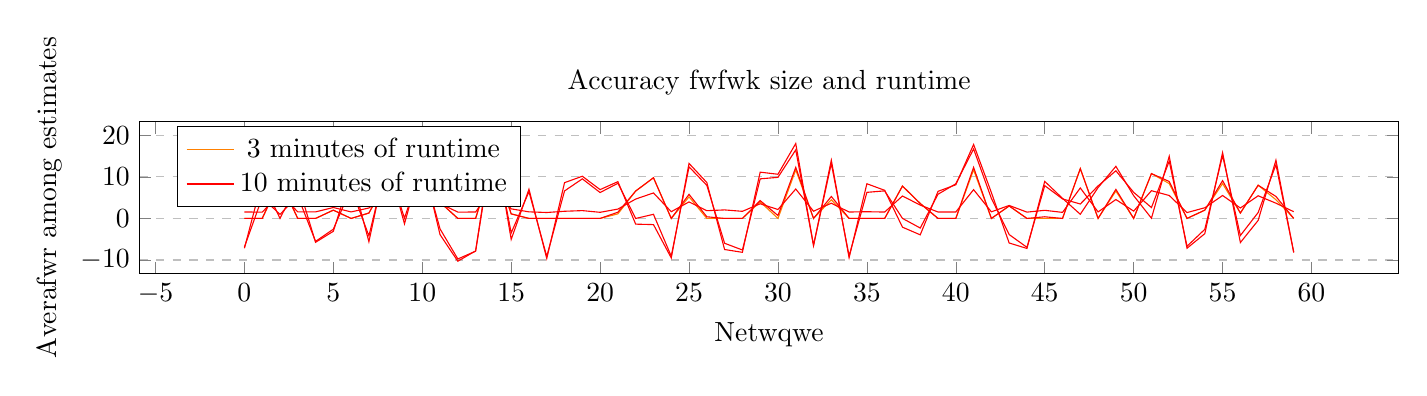
\begin{tikzpicture}
		\begin{axis}[
			title={Accuracy fwfwk size and runtime},
			xlabel={Netwqwe},
			ylabel={Averafwr among estimates},
			%xmin=0, xmax=0.25,
			%ymin=0.0001, ymax=1.0,
			%ymode=log,
			%xtick={0,0.05,0.1,0.15,0.2,0.25},
			%ytick={0,20,40,60,80,100},
			%yticklabel=$\pgfmathprintnumber{\tick}\%$,
			legend pos=north west,
			ymajorgrids=true,
			grid style=dashed,
			xticklabel style={/pgf/number format/fixed},
			width = 500,
			height = 100
		]
	%	\addplot [domain=5:15,dotted] {20+exp(exp(x/6.2))};
		\addplot[color=orange] coordinates {
(0,0.0)(1,0.0)(2,9.1)(3,0.0)(4,0.0)(5,2.0)(6,0.0)(7,1.3)(8,8.8)(9,7.2)(10,7.2)(11,3.9)(12,0.0)(13,0.0)(14,13.5)(15,1.1)(16,0.0)(17,0.0)(18,0.0)(19,0.0)(20,0.0)(21,1.1)(22,6.6)(23,9.8)(24,0.0)(25,5.2)(26,0.0)(27,0.0)(28,0.0)(29,4.0)(30,0.0)(31,11.7)(32,0.0)(33,4.5)(34,0.0)(35,0.0)(36,0.0)(37,7.8)(38,3.6)(39,0.0)(40,0.0)(41,11.7)(42,0.0)(43,3.0)(44,0.0)(45,-3.5527136788e-15)(46,0.0)(47,12.0)(48,0.0)(49,6.6)(50,0.0)(51,10.8)(52,8.4)(53,0.0)(54,2.0)(55,8.4)(56,1.3)(57,8.0)(58,4.5)(59,0.0)
			}node[pos=0.8](endofplotsquare){} ;
\addplot[color=red] coordinates {
(0,0.0)(1,0.0)(2,9.1)(3,0.0)(4,0.0)(5,2.0)(6,0.0)(7,1.3)(8,9.2)(9,7.2)(10,7.7)(11,3.9)(12,0.0)(13,0.0)(14,14.3)(15,1.1)(16,0.0)(17,0.0)(18,0.0)(19,0.0)(20,0.0)(21,1.5)(22,6.6)(23,9.8)(24,0.0)(25,5.8)(26,0.4)(27,0.0)(28,0.0)(29,4.3)(30,0.7)(31,12.3)(32,0.0)(33,5.3)(34,0.0)(35,0.0)(36,0.0)(37,7.8)(38,3.6)(39,0.0)(40,0.0)(41,12.3)(42,0.0)(43,3.0)(44,0.0)(45,0.4)(46,0.0)(47,12.0)(48,0.0)(49,7.0)(50,0.0)(51,10.8)(52,8.9)(53,0.0)(54,2.0)(55,9.1)(56,1.3)(57,8.0)(58,5.3)(59,0.0)
			}node[pos=0.8](endofplotsquare){} ;
\addplot[color=red] coordinates {
(0,1.55828042368)(1,1.51378390307)(2,5.89724242335)(3,1.59739817416)(4,1.57241703752)(5,2.63639541592)(6,1.57069425998)(7,2.51460535369)(8,5.74807237466)(9,5.11662397151)(10,4.80678912775)(11,3.57889142294)(12,1.53225542092)(13,1.5425)(14,7.77515548206)(15,2.30535057629)(16,1.58617144777)(17,1.42985992276)(18,1.72786663416)(19,1.88368851843)(20,1.47670862584)(21,2.25631008495)(22,4.67099674417)(23,6.13825734374)(24,1.6231804078)(25,3.98224349486)(26,1.86675135007)(27,2.05501579969)(28,1.71191569622)(29,3.5327863356)(30,2.14971927553)(31,7.08526583034)(32,1.73885278506)(33,3.66961403525)(34,1.54504123854)(35,1.61881930148)(36,1.53936502151)(37,5.40530360158)(38,3.21470257348)(39,1.54782934243)(40,1.55586928552)(41,6.93162774423)(42,1.59214090811)(43,3.13069125373)(44,1.52252011234)(45,1.95573629336)(46,1.45944830637)(47,7.34113270311)(48,1.56745675299)(49,4.55532447479)(50,1.76883332971)(51,6.68234280265)(52,5.52640188853)(53,1.41522175123)(54,2.57218198959)(55,5.52717325397)(56,2.51489487224)(57,5.45634022188)(58,3.67352365999)(59,1.62293691949)
			}node[pos=0.8](endofplotsquare){} ;
\addplot[color=red] coordinates {
(0,-7.18657325906)(1,9.10936734333)(2,0.0154577001048)(3,8.35657525165)(4,-5.74466052641)(5,-3.09706024461)(6,10.4972354392)(7,-5.60324832146)(8,14.4081814454)(9,-1.29326390424)(10,14.1741616708)(11,-3.91213868856)(12,-10.3012294742)(13,-7.81557972083)(14,20.2475741297)(15,-5.05061832051)(16,7.03476589515)(17,-9.64560698554)(18,8.613763694)(19,10.1659071297)(20,6.94014908481)(21,8.86171162256)(22,-1.37529357656)(23,-1.48409903067)(24,-9.50790609341)(25,13.2578338469)(26,8.64983465525)(27,-7.48625692709)(28,-8.16023099149)(29,11.1489499337)(30,10.6422803208)(31,18.0427826677)(32,-6.50988104492)(33,14.0355928651)(34,-9.45755431236)(35,8.35509633846)(36,6.77701477294)(37,-2.10216486564)(38,-3.94877305098)(39,6.52639477794)(40,8.10864532472)(41,17.8175448548)(42,6.23389404874)(43,-5.91451154279)(44,-7.22855975946)(45,8.92696941)(46,4.83527762134)(47,1.00404500911)(48,7.42801949162)(49,12.550966324)(50,5.48206864098)(51,0.0556137309222)(52,14.9822780268)(53,-7.17680121495)(54,-3.67178196341)(55,15.8712704166)(56,-5.80610585086)(57,-0.468133357491)(58,14.034338542)(59,-8.20772999475)
			}node[pos=0.8](endofplotsquare){} ;
\addplot[color=red] coordinates {
(0,-6.89493154762)(1,5.04268903319)(2,0.972028769841)(3,5.41843253968)(4,-5.52792989418)(5,-2.58917237855)(6,7.31814732143)(7,-4.20128075397)(8,13.4425248016)(9,0.0417471891534)(10,12.9921789021)(11,-2.52101636905)(12,-9.75983912037)(13,-7.88896676587)(14,18.9899358466)(15,-3.49210664683)(16,6.43908779762)(17,-9.16015612975)(18,6.62748875661)(19,9.53488839286)(20,6.23878769841)(21,8.46800462963)(22,-0.00978968253968)(23,0.996877314815)(24,-9.10146626984)(25,12.429577877)(26,7.97395585317)(27,-5.97840724206)(28,-7.59884887566)(29,9.53766815476)(30,9.89875049603)(31,16.5072901786)(32,-6.49119890873)(33,13.2445252976)(34,-9.02564763709)(35,6.28314980159)(36,6.63935796958)(37,0.013751984127)(38,-2.30903339947)(39,5.83215839947)(40,8.34694874339)(41,16.7391850198)(42,4.83128108466)(43,-3.88587334656)(44,-6.95309573413)(45,7.89512946429)(46,4.70475016534)(47,3.47914276696)(48,7.83959460678)(49,11.4769315476)(50,6.29048048942)(51,2.62045171958)(52,13.8020848214)(53,-6.70164649471)(54,-2.62177959656)(55,15.1610186839)(56,-4.11308068783)(57,1.42724255952)(58,12.9501597222)(59,-8.12579963324)
			}node[pos=0.8](endofplotsquare){} ;
\addlegendentry{3 minutes of runtime}
\addlegendentry{10 minutes of runtime}
		\end{axis}
		\end{tikzpicture}
		%\vspace{-18pt}
		\caption{Averafwwfwetworke minutes rufektop computer.}
		\label{fig:experiment_graph1}
    \end{figure}



